%%% CBC SEARCH %%%
% Gravitational Wave data
%    h = s + n
% Signal Model
%    Waveforms
% Noise Model
%    PSD
% Search Methods
%    Matched Filter
%    Phase Maximisation
%    Template Bank
%    Signal Consistency Tests
%    Exponential Noise Model
%    PSD Variation
%    Coincidence Tests
%        Simple One
%        PhaseTD
%    Ranking Statistic
% PyCBC
%    Offline vs Live
%    Low-Latency Detection
%    SNR Optimization
% Gravitational-Wave Observations to date



% Chapter Introduction

Gravitational wave search pipelines, such as PyCBC, play a critical role in analyzing data from detectors to identify gravitational wave signals, both in real-time (live) and in post-processing (offline). This chapter develops the theoretical foundation for these search pipelines and explores the techniques employed in gravitational wave detection. Emphasis is placed on the PyCBC pipelines---PyCBC Offline and PyCBC Live---both of which were extensively utilized and further developed as part of this thesis.

\section{\label{2:sec:gw-data}Gravitational Wave Data}

Gravitational wave observatories produce a dimensionless strain time-series, $s(t)$, which is composed of detector noise, $n(t)$, and, when present, an astrophysical gravitational wave signal, $h(t)$. This relationship is expressed as:
%
\[
    s(t) =
    \begin{cases}
        n(t), & \text{if no signal is present}, \\
        n(t) + h(t), & \text{if a signal is present}.
    \end{cases}
\]
%
The primary objective of gravitational wave search pipelines is to extract $h(t)$ from $s(t)$, isolating the astrophysical signal from the background noise.



\subsection{Constructing Frequency-Domain Signals}

Although the raw data from gravitational wave detectors are delivered as time-series strain data, it is often desirable to perform the signal analysis in the frequency domain. This is because many gravitational wave search algorithms operate more efficiently in the frequency domain, where the noise characteristics of the detector and the signal structure can be more easily distinguished.

To convert the time-domain waveform $h(t)$ into the frequency domain $h(f)$, we apply the Fourier transform. The stationary phase approximation (SPA) is a common technique used to analytically compute the Fourier transform of certain types of signals, especially those with a slowly varying amplitude and rapidly varying phase, as is often the case for inspiral signals from CBC sources.

In gravitational wave data analysis, the stationary phase approximation (SPA) is often used to transform the time-domain signal $h(t)$ into its frequency-domain counterpart $h(f)$. The key idea behind the SPA is that the phase of the signal varies much more rapidly than its amplitude, which allows for an efficient approximation of the Fourier transform.

Consider a time-domain gravitational wave signal $h(t)$ of the form:
\begin{equation}
    h(t) = A(t) \cos(\phi(t)),
\end{equation}
where $A(t)$ is the slowly varying amplitude and $\phi(t)$ is the rapidly varying phase. In compact binary coalescences, the phase $\phi(t)$ is dominated by the orbital evolution of the binary system.

To obtain the frequency-domain waveform $h(f)$, we perform a Fourier transform of $h(t)$. The stationary phase approximation allows us to approximate this Fourier transform by focusing on points in time where the phase is stationary, meaning that the derivative of the phase with respect to time is equal to the angular frequency, $\omega = 2 \pi f$. Specifically, this occurs when:
\begin{equation}
    \frac{d\phi(t)}{dt} = 2 \pi f.
\end{equation}
Let \( t' \) be the time at which this condition is satisfied, i.e., 
\[
    \frac{d\phi(t')}{dt} = 2 \pi f.
\]

The frequency-domain approximation of the signal, $h(f)$, is then given by:
\begin{equation}
    h(f) \approx \frac{A(t')}{\sqrt{\left| \frac{d^2 \phi(t')}{dt^2} \right|}} e^{i \left( 2 \pi f t' - \phi(t') \right)}.
\end{equation}
Here, \( A(t') \) is the amplitude at the stationary phase point, and \( \frac{d^2 \phi(t')}{dt^2} \) is the second derivative of the phase at the stationary time \( t' \). This approximation captures the essential features of the signal in the frequency domain, with the rapid oscillations of the phase dictating the frequency content of the waveform.

The SPA provides an efficient way to model the inspiral phase of compact binary coalescence signals, which is particularly useful for search pipelines analyzing data in the frequency domain.


\subsection{Waveform models}

Two primary waveform families are commonly used in CBC signal modeling:
\begin{itemize}
    \item \textbf{Inspiral-Merger-Ringdown (IMR) Models:} These models, such as IMRPhenom and SEOBNR, describe the entire evolution of a binary coalescence, from the inspiral phase through the merger and into the post-merger ringdown. These models are widely used in the analysis of gravitational wave signals.
    \item \textbf{Effective-One-Body (EOB) Models:} These models provide a physically motivated description of the two-body problem in general relativity and can be extended to model the inspiral, merger, and ringdown of binary systems. SEOBNR is one such EOB model, extensively used in data analysis pipelines like PyCBC.
\end{itemize}

In this work, we focus on the use of IMR models, as they provide a complete description of the waveform throughout the entire coalescence process.


\section{\label{2:sec:noise-model}Modelling Gravitational-Wave Data Noise}

Gravitational wave data noise 

\section{\label{2:sec:search-methods}Search Methods}

\subsection{\label{2:sec:matched-filter}Matched Filter}

Using GR, we can produce waveforms which represent a \gw in our photodetector output. Knowing what we are looking for allows us to use matched filtering, a signal processing technique where a known signal is correlated with data to
obtain a signal-to-noise ratio (SNR) informing us of the likelihood of the waveform being in the data

To being we can the data as a sum of a signal and noise:

\begin{equation}
   s(t) = h(t) + n(t)
   \label{2:eqn:s_h_n}
\end{equation}

Where $s$ is the data, $h$ is a signal (in this case, a real \gw signal) and $n$ is the noise. Using a template of the signal, we can use matched filtering to find the signal within our data.

The matched filter is defined as \cite{PyCBC:2016}:

\begin{equation}
   \rho^2(t) = \frac{(s|h)^2}{(h|h)}
   \label{2:eqn:matched_filter}
\end{equation}

The weighted inner product of the data, $s$, and the signal, $h$, in the frequency domain producing a signal-to-noise ratio (SNR), $\rho^2(t)$, in the time domain. We define the inner product:

\begin{equation}
   (s|h)(t) = 4 \Re \int^{+\infty}_{-\infty} \frac{\tilde{s}(f) \tilde{h}^*(f)}{S_n(f)} e^{2 \pi i f t} df
   \label{2:eqn:inner_product}
\end{equation}

A tilde, e.g. $\tilde{s}(f)$, denotes a Fourier transformed version of the variable.

\begin{equation}
   \tilde{s}(f) = \int^{+\infty}_{-\infty} s(t) e^{-2 \pi i f t} dt
   \label{2:eqn:fourier_transform}
\end{equation}

In equation \ref{2:eqn:inner_product} we have Fourier transformed data, $\tilde{s}(f)$, and a Fourier transformed signal, $\tilde{h}(f)$.

On the denominator within the integral in equation \ref{2:eqn:inner_product} $S_n(f)$ is the power spectral density (PSD) of the detector noise:

\begin{equation}
   \langle \tilde{n}(f) \tilde{n}(f') \rangle = \frac{1}{2} S_n(f) \delta(f-f')
   \label{2:eqn:PSD}
\end{equation}

The angle brackets denote averaging over noise realizations, $n$ is stationary Gaussian detector noise and $\delta$ is the Dirac delta function.

These equations build a tool that allows us to analyse a data to look for a signal. One requirement is that we must know the signal we are looking for before we search for it. We can create a template of our signal, referred to as a waveform. We then matched filter our data with the waveform and search through the resulting SNR timeseries for a peak, indicating the presence of the signal.

\subsection{\label{2:sec:phase-maximisation}Phase Maximisation}

Furthermore, the matched filter maximises the amplitude of the \gw signal and we have the ability to maximise over the phase of the signal by using an altered version of the matched filter:

\begin{equation}
   \text{$\rho^2_{\Phi,max}(t) = \frac{(s|h)^2 + (s|h_{\pi/2})^2}{(h|h)}$ where $\tilde{h}_{\pi/2}(f) = i \tilde{h}(f)$}
   \label{2:eqn:phase_mf}
\end{equation}

Where $\tilde{h(f)}$ and $\tilde{h}_{\pi/2}(f)$ are orthogonal phases of our template.

\subsection{\label{2:sec:template-bank}Template Bank}

Our waveform template bank will be only 5 parameters: the two masses, the two free spins and, the time of coalescence. We must create a bank of waveform templates describing all the possible signals and template density of the bank needs to be fine-tuned in order to ensure two things: our template bank covers the parameter space well enough to find all signals and our template bank isn't so large we are wasting computational time and resources \cite{Owen_Sathya:1999}.

\subsection{\label{2:sec:signal-consistency}Signal Consistency Tests}

\subsection{\label{2:sec:template-fits}Exponential Noise Model}

\subsection{\label{2:sec:psd-var}PSD Variation}

\subsection{\label{2:sec:coincidence-test}Coincidence Tests}

\subsection{\label{2:sec:ranking-statistic}Ranking Statistic}
% Searches need a ranking statistic to map to FAR
% We will discuss the PyCBC ranking statistic in more detail later on
% Signal Consistency Tests
% Astro signal rates and that
% The optimal ranking statistic -> the ranking statistic we have
The ranking statistic is a measure of confidence that a signal originated from an astrophysical source as opposed to noise in the detectors. We use the ranking statistic to calculate a false alarm rate which informs us of the number of events per unit time that will originate from noise only. There must be a balance struck when choosing a false alarm rate at which events are determined to be real, require a very small false alarm rate and you will potentially exclude real events from a catalogue and allow too high of a false alarm rate and you will potentially include noise in the catalogue. In this section we will describe the different components which make up the ranking statistic.

%%%%%%%%%%%%%%%%%%%%%%%% TAKEN FROM PYCBCLIVE
Each trigger in an interferometer (H1 and L1) will produce an \verb|SNR| ($\rho$), $\chi^{2}$, $\chi^{2}$ degrees of freedom ($\chi^{2}_{dof}$) and Sine-Gaussian $\chi^{2}$ (\verb|sg_chisq|). To calculate the new SNR ($\rho_{new}$) for each trigger we must firstly convert $\chi^{2}$ to reduced-$\chi^{2}$ using the degrees of freedom which needs to itself be converted from the degrees of freedom saved in the Live trigger files:
%
\begin{equation}
\text{dof} = 2 \cdot \chi^{2}_{dof} - 2,
\end{equation}
%
\begin{equation}
  \chi_{reduced}^{2} = \frac{\chi^{2}}{\textrm{DOF}} = \frac{n}{2n - 2} \sum_{i=1}^n \left(\frac{\rho}{\sqrt{n}} - \rho_{bin,i}\right)^2.
  \label{2:eqn:chi_squared}
\end{equation}
%
\begin{equation}
\rho_{rw} =  \left\{  \begin{array}{l@{\quad}cr} 
\rho & \mathrm{if} & \chi_{r}^{2} < 1, \\  
\rho [(1 + (\chi_{r}^{2})^3)/2]^{-\frac{1}{6}} &  \mathrm{if} & \chi_{r}^{2} \ge 1,   
\end{array}\right.
\label{2:eqn:allen-reweighting}
\end{equation}
%
\begin{equation}
\rho_{\text{new}} = 
\begin{cases} 
\rho_{\text{rw}} & \text{if } \text{sg\_chisq} \leq 4, \\  
\rho_{\text{rw}}  / \left(\frac{\text{sg\_chisq}}{4}\right)^{0.5} & \text{if } \text{sg\_chisq} > 4.
\end{cases}
\label{2:eqn:sg-reweighting}
\end{equation}

Another consideration in the ranking statistic calculation when comparing the old statistic to the new statistic is how the $\rho_{new}$ for each detector is accounted for in the ranking statistic calculation. The old statistic is composed of two quantities, \verb|rstat|, which is the single detector $\rho_{new}$ and, \verb|logr_s|, which is the log of the expected signal rate. \verb|rstat| is calculated by summing the squares of the $\rho_{new}$ from each detector,
%
\begin{equation}
    \textbf{rstat} = \rho_{new, H1}^{2} + \rho_{new, L1}^{2}
\end{equation}
%
which then to find the total ranking statistic is added to $2 \times$ the log signal rate and square rooted,
%
\begin{equation}
    \textbf{cstat} = (\textbf{rstat} + 2 \cdot \textbf{logr\_s})^{\frac{1}{2}} \ .
\end{equation}
%
The new statistic simply takes the log signal rate, \verb|logr_s|, and subtracts the combined lognoiserate, \verb|ln_noise_rate|,
%
\begin{equation}
    \textbf{loglr} = \textbf{logr\_s} - \textbf{ln\_noise\_rate}
\end{equation}
%
where the combined lognoiserate is calculated in equation~REMOVED.

We can directly compare how $\rho_{new}$ manifests in both of these equations. In the old statistic we are summing the squares of the $\rho_{new}$ from each interferometer and then square rooting after adding the contribution from the signal rate. In the new statistic we are simply adding the $\rho_{new}$ from each interferometer together (after applying the fits values). Due to this the old statistic will prefer higher SNR ratios between the two interferometers whereas the new statistic will favour equal SNRs.

For the old statistic, the quadrature sum of the SNRs will maximise the equation,
%
\begin{equation}
    a^{2} + b^{2} = (a + b)^{2} - 2ab
\end{equation}
%
where the difference between $a$ and $b$ is largest (neither $a$ or $b$ can be $0$ in our example because a coincidence detection requires both detectors to pass the minimum threshold). Therefore \verb|rstat| will be largest where the SNR ratio is greatest. In contrast, the new statistic will naturally favour equal SNRs as the search attempts to maximize the sum of the lognoises and not the squared sums when searching for coincidence pairs.

To visualise this difference we can plot the distribution of H1 and L1 SNR values and their coincident detector ranking statistic values. In both of these figures we neglect a changing signal rate and focus solely on the SNR contribution to the single detector ranking statistic.
%
%%%%%%%%%%%%%%%%%%%%%%%%%%%%%%%%%%%%%

\section{\label{2:sec:pycbc-live}PyCBC}

% Overarching points:
% - State of the field before my work
% - Overview of PyCBC Live in O3
% - Avoid talking about new developments

% What to talk about in this section:
% - Offline vs Live differences
% - Difference in computation of ranking statistic
% - How is ranking computed in Live
% -     Focus on methodology instead of code
% - O3 it wasn't able to cmopute some of the quantities that offline could
% -     Particularly things based on bulk statistics
% - Results in PyCBC Live being less sensitive
% -     List number of offline detections vs num live detections
% -     R&P paper demonstrated PyCBC Live is the most sensitive pipeline in all regions of parameter space in O3
% -     But gstlal had more events than pycbc (cross compare numbers and look at other pipelines)

%

% Introduction to the section

This section combines the previously discussed techniques into an end-to-end pipeline used to detect gravitational waves. We will discuss primarily the PyCBC Live real time search for gravitational waves and how this search differs from the PyCBC offline search for gravitational waves including the limitations and the methodology differences to overcome these limitations.

\section{\label{2:sec:offline-vs-live}Offline vs Live}
% Differences in offline vs live

The search for gravitational waves occurs over two different time-scales. There is a "real-time" live search and an offline "post-detection" search, these searches have broadly the same goals---to detect gravitational waves---however they have different limitations, especially in the case of the live searches. Where the offline search has more time and potentially computing power available to probe the data more deeply, the live search is capable of rapidly sending information of potentially electromagnetically bright events to other astronomical observatories to perform multi-messenger astronomy.

Currently PyCBC operates three searches on data from the fourth observing run: the PyCBC Live Full-Bandwidth search, with $\sim$730k templates in the template bank; the PyCBC Live Early Warning search, with a smaller $\sim$9k template bank comprised of only electromagnetically bright frequency truncated signals and the PyCBC Offline search which uses another large template bank of $\sim$696k templates to find all gravitational wave signals in the data.

This section will describe the PyCBC Live search in greater detail, focussing on the optimizations and unique components that differ it from the offline search and how these help to improve our detection of gravitational waves. The full bandwidth search is being described in these sections, the early warning search varies every so slightly but not enough to require distinctions to be made.

\subsection{\label{2:sec:low-latency-detection}Low-Latency Detection}
%
\begin{figure}
    \centering
    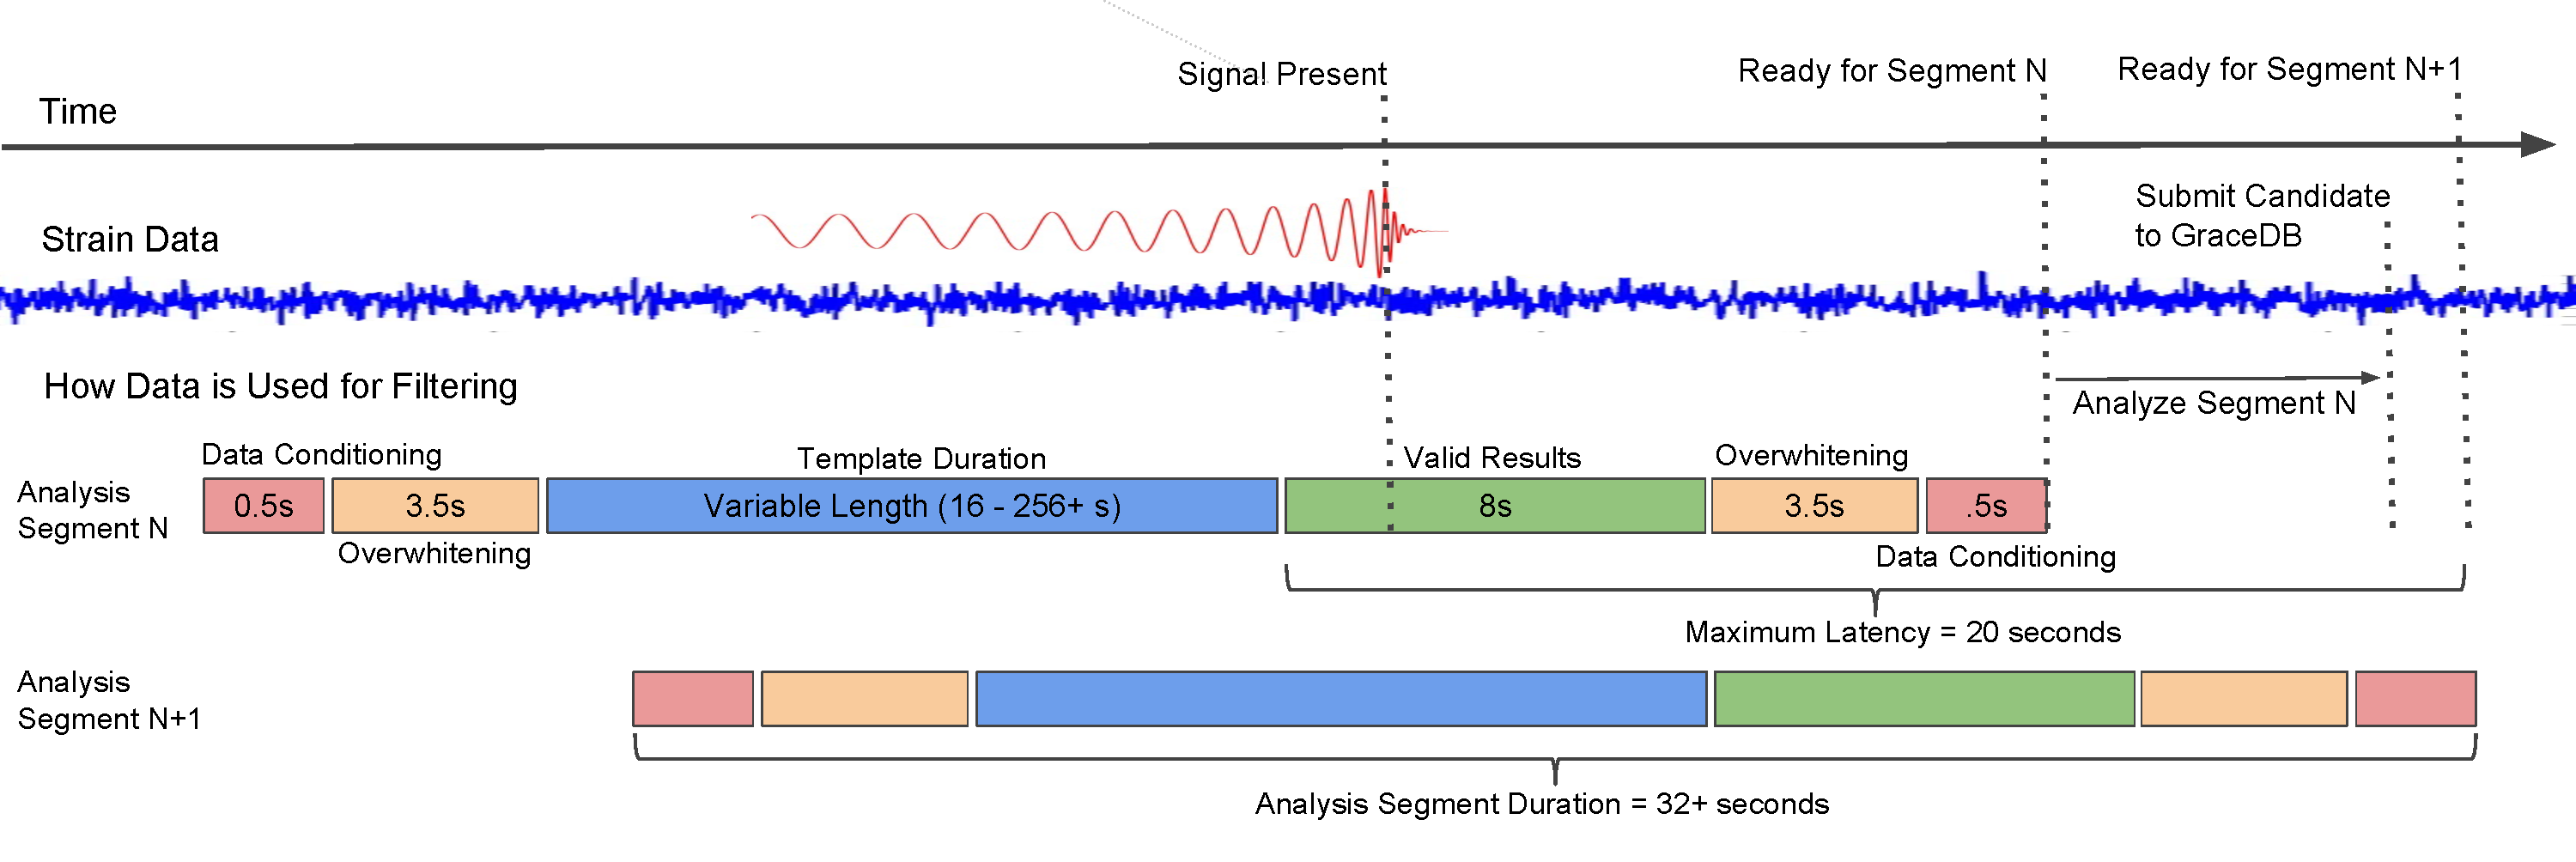
\includegraphics[width=1.0\linewidth]{images/2_searches/live_latency_diagram.pdf}
    \caption{Caption}
    \label{2:fig:live_latency_diagram}
\end{figure}
%
The PyCBC Live search aims to detect all gravitational waves in real time. This is a feat of software engineering to obtain the gravitational wave data, perform the matched filtering of hundreds of thousands of templates, perform signal consistency tests and output an approximate sky map within tens of seconds of the merger of the gravitational wave passing through the detectors.

The live search is distributed over 151 computing nodes and these are all connected through a message passing interface which tracks the individual search nodes. The main ranked node will receive messages from each of these nodes and distribute information and jobs to all the nodes. For example, when a node running a matched filter on H1 data finds a trigger and a node running a matched filter on L1 data finds a trigger, these triggers are sent back to the rank 0 node which then assigns another node to perform the coincidence tests as part of the ranking statistic to determine if this trigger was a real gravitational wave event.

The template bank of 730 thousand template distributed throughout the nodes and pre-generated in memory so the matched filters do not have to rely on generating the templates every time new data arrives. The template bank is shuffled into a random order so that the distribution of `long' and `short' templates is randomly distributed throughout the nodes. If a single node has all the long templates it will take longer to perform the matched filters than the nodes with the short templates and this can introduce lagging effects if the search is being held up by a single node.

The live search holds a continuous buffer of data where the newest eight seconds of data are added to the front and push the oldest eight seconds of data out of the buffer. The data is then matched filtered with the template bank and each node reports on the triggers that have been found. The hope with the search is that all of this processing can happen before the next eight seconds of data arrives at the detector. (PLOT: PYCBC LIVE LAG PLOT DIAGRAM THING)

\subsection{\label{2:sec:snr-optimization}SNR Optimization}

We upload potential detections of gravitational wave events to a central public database called GraceDB. These events are then used by astronomers to observe potential electromagnetic counterparts. We want to report the best information we can and produce the most accurate sky map. Increasing the SNR of the event is an easy way to improve this, having a better matching template to the signal will do this. (REWRITE).

The SNR optimization module of PyCBC Live takes a gravitational wave event and uses optimization functions to rapidly optimize the gravitational wave parameters to retrieve small fractions of improvement to the SNR. The original SNR of the event is limited by the template bank placement and the SNR optimizer allows a much finer exploration of the local parameter space to the best found template in the template bank. (ADD PLOT SHOWING TEMPLATE BANK WITH TEMPLATES NEARBY THE ACTUAL PARAMETER VALUES AND SNR IMPROVEMENT).

\subsection{\label{2:sec:live-ranking-statistic}Ranking Statistic}

The PyCBC Live ranking statistic run in the third observing run and the first half of the fourth observing run was very simple, only taking into account the Allen chisq, sine-gaussian chisq and phasetd. These are basic signal consistency tests for single detector checks, re-ranking the snr depending on how the morphology of the snr evolves over the signal. In coincidence the ranking statistic only looks for phase and template consistency for the two triggers and a time coincidence so that both detector triggers fall in light time travel time.



% Removed from pycbclive.tex
This chapter details the changes made to the PyCBC Live ranking statistic to improve on the original ranking statistic used in the third and fourth observing runs and detailed in~\ref{2:sec:live-ranking-statistic}. The two additions that were made to the ranking statistic were the inclusion of PSD variation, to track the non-stationary of the detector noise, and adding template fits to the statistic to weigh triggers based on their previously measured SNR distribution.

In this chapter we introduce the PyCBC Live search for CBC signals and the improvements made to the PyCBC Live search's ranking statistic to improve the sensitivity of the search and the confidence of our gravitational wave detections. The PyCBC Live search has been operational since the 2018~\cite{PyCBC_Live:2018} and has been in constant operation since, contributing to the 2nd, 3rd and 4th observing runs and detecting over 200 gravitational wave events. The PyCBC Live search processes gravitational wave detector data using techniques described in section~REMOVED however, there are a number of optimizations and new techniques used to enable to low-latency rapid detection of gravitational wave events in close to real time.

PyCBC Live uses a ranking statistic post-detection of a gravitational wave event candidate which provides a numerical confidence in the event being real. This number is referred to as the `False Alarm rate' (FAR) and is measured in units of events per unit time (typically per year or Hertz). The inverse of the false alarm rate (IFAR) is commonly used and is typically measured in units of years. The false alarm rate tells us how often a candidate event would be observed due to random noise in the absence of a real astrophysical signal. IFAR can be thought of as the expected time interval between random noise events that could produce a signal resembling the observed candidate event. A higher IFAR indicates a longer expected waiting time between false alarms.

The LVK places a limit on the IFAR of a signal before it can be determined to be real. The limit has to be placed to balance the sensitivity of a search and the purity of a gravitational wave catalogue. As a quick example, if the IFAR limit is set to 1 year. Then one might expect to see one event per year in the catalog purely due to noise.

We begin this chapter by detailing the components that make up the ranking statistic and then the new components of the improved ranking statistic and how these are derived and used.

\section{\label{2:sec:current-detections}Gravitational-Wave Observations to date}
